%% arara: lualatex: {draft: yes}

%% arara: lualatex
%% arara: lualatex

% arara: lualatex
% arara: biber
% arara: lualatex
% arara: lualatex
%% arara: clean: { extensions: [ aux, log, bbl, bcf, blg, listing, out, run.xml, toc, upa, upb, pdf ] }

% classe com as customizações -------------------------------------------------
\documentclass{minicursoUFRB}

% meus comandos ---------------------------------------------------------------
% \begin{cita} ...
% \begin{codigo}{titulo}{\lapis} ...
% \begin{codeLaTeX} ...
% \begin{atencao}{titulo}{\exclamacao} ...
% \tcboxC{}
% \nota{}
% \lualatex
% \pdflatex
% \Overleaf
% \mn{} ou \sidenote{} --> texto normal
% \en{} --> pequeno
% \sn{} --> pequeno e itálico
% \textbs{} ---> texto em negrito e sem serifa 
% \textas{} ---. texto em azulUFRB sem serifa
% \hrefB{}{} --> negrito (com dourado)
% \hrefA{}{} --> negrito com azulUFRB

%==============================================================================
% Início do Documento 
%------------------------------------------------------------------------------
\begin{document}
%
  \capa
%
  \thispagestyle{empty}
  \tableofcontents
%
  \flushbottom
  \newpage
%
  %==============================================================================
% Introdução ao texto
%==============================================================================
\thispagestyle{empty}

\section*{Bate-papo Inicial}

\begin{marginfigure}
  \centering
  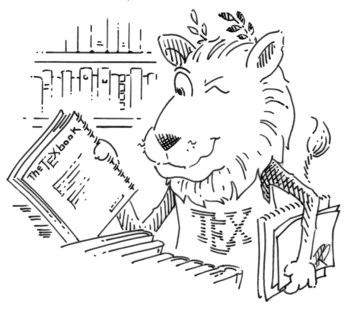
\includegraphics[width = \linewidth]{ctan_lion_350x350}
\end{marginfigure}

Se você optou por ler esse material, vá até o fim!
O \LaTeX\ pode ser para você uma ferramenta extremamente agradável para produção
tipográfica, a nível profissional, de suas futuras notas de aula; monografias,
dissetações ou teses; listas de atividades; partituras; marcações no xadrez; etc.

Não pretendo abordar muita coisa, confesso.

Fui incumbido de ministrar, em pouco mais de 3\unit{\hour}, uma introdução ao 
\LaTeX.

\begin{codigo}{Exemplo de preâmbulo}{\lapis}
% arara: lualatex: {options: ['--output-directory=docs_saida']}

% classe do documento -------------------------------------------------------
\documentclass[12pt]{article}

% pacotes carregados --------------------------------------------------------
\usepackage{mathtools, amsfonts, amsthm}

% configurações do título ---------------------------------------------------
\title{\textbf{Título}}
\author{Ícaro Vidal Freire}
\date{\today}

%============================================================================
% Início do Documento
%----------------------------------------------------------------------------
\begin{document}
%
  \maketitle % produz a saída do título
%
\begin{abstract}
  Pequeno resumo.
\end{abstract}
%
\section{Primeira Seção}

Olá \LaTeX!
%---------------------------------------------------------------------------- 
\end{document}
%============================================================================
\end{codigo}

%------------------------------------------------------------------------------
\newpage
%
  \pagestyle{fancynotes}
%
  \part{A Arte de Nomear as Coisas}	
%
    \section{A Seiva da Árvore \ldots}\label{sec:seiva} %==========================

\begin{margintable}\vspace{.8in}\footnotesize
  \caption{Sumário da \textsc{Part I}} 
  \medskip  
  \begin{tabularx}{\marginparwidth}{|X}
    \textbf{\sffamily \textcolor{azulUFRB}{Seção}~\ref{sec:seiva}}.    {\sffamily A seiva da árvore}                  \\
    \textbf{\sffamily \textcolor{azulUFRB}{Seção}~\ref{sec:usando}}.   {\sffamily Sim\ldots mas como eu uso?}         \\
    \textbf{\sffamily \textcolor{azulUFRB}{Seção}~\ref{sec:overleaf}}. {\sffamily Overleaf: um editor online notável} \\
  \end{tabularx}
\end{margintable}

Lembro-me da primeira vez que vi o nome \LaTeX{} \ldots

Foi em uma chamada de um minicurso de alguma "semana de matemática" da 
universidade que fiz graduação.
O título era algo assim: "Introdução ao \LaTeX".

Eu estava a um semestre de concluir a graduação e pensei: 
\textit{
  "Rapaz \ldots acho que eles erraram esse minicurso. 
  Pra quê estudar látex em Matemática? 
  Isso está mais para Geografia."
}

Sim! 
Eu pensei que estavam falando daquela substância espessa e branca que sai de 
algumas plantas (seringueira, por exemplo)!

Então, vamos deixar as coisas claras: não estamos falando de látex, mas de \LaTeX.

\begin{atencao}{Como pronunciar corretamente?}{\exclamacao}
  Aliás, como se pronuncia a palavra \LaTeX?\\
  Existem, pelo menos, duas maneiras de pronunciarmos, corretamente, essa palavra:
  "\textit{LeiTéc}" ou "\textit{LaTéc}", ou seja, o som de \TeX{} ("Téc") é o 
  mesmo que na palavra "\textit{tec}nologia". 
  Particularmente, adoto a segunda opção.
  Evite, por amor a Deus, falar "\textit{Látecks}".
\end{atencao}

\begin{marginfigure}
  \centering
  \caption{Isso é látex, não \LaTeX}
  \medskip
  \href
  {
    https://www.globo.com/GloboRural/0,6993,EEC1703411-1935,00.html
  }
  {
    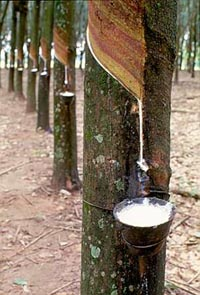
\includegraphics[width = 0.75\linewidth]{seringueira.jpg}
  }

  {\small \textbf{Fonte:} \sffamily Globo Rural}
\end{marginfigure}

Falando nisso, essa palavra \TeX{} não está destacada de forma aleatória! 
Ela foi idealizada como sendo a junção de três letras gregas: $\tau\epsilon\chi$.
\footnote{%
  $\tau$ (tau), $\epsilon$ (épsilon) e $\chi$ (chi)
}
Esse núcleo grego gera palavras como \textit{arte} ($\small\tau\epsilon\chi\nu\eta$) 
ou mesmo \textit{tecnologia} ($\small\tau\epsilon\chi\nu o \lambda o \gamma\iota\alpha$).
Daí vem o espírito da palavra \TeX: unir uma arte (a tipografia) com a tecnologia 
(programação) para produzir documentos com uma beleza realmente ímpar.

Na realidade, para falarmos com propriedade sobre \LaTeX, precisamos tangenciar 
o \TeX.

\subsection{Diferenciando os nomes} %------------------------------------------

Tudo começou quando \href{https://pt.wikipedia.org/wiki/Donald_Knuth}{Donald Ervin Knuth} 
queria qualidade nos elementos tipográficos de seus livros, principalmente na 
escrita matemática. 
Ele então criou, em meados da década dos anos 70, um sofisticado programa para a 
composição tipográfica de textos científicos e uma alternativa quase necessária 
para edição de textos com conteúdo matemático. 
Nasceu o \TeX. 
Em suas próprias palavras:

\begin{cita}
  \TeX{} é destinado para a criação de belos livros - e, especialmente, para os 
  livros que contêm grande quantidade de matemática.
\end{cita}

Todavia, ao que parece, essa linguagem de programação não era tão acessível 
\sout{a meros mortais como nós}, por conter diversos parâmetros relativos ao 
formato final do texto \ldots
Bom, vamos falar a verdade: dava muito trabalho para digitar o que você queria 
simplificar.
Isso porque o \TeX{} era formado por objetos denominados "primitivos" e toda 
estruturação do texto deveria ser feita por meio deles.
O próprio Knuth criou um conjunto de macros\nota{
  Uma \textit{macro} (abreviação para macroinstrução), em ciência da computação, 
  é uma regra ou padrão que especifica como uma certa “sequência de entrada” 
  deve ser mapeada para uma substituição de “sequência de saída” de acordo com 
  um procedimento definido.
}, ou seja, um mapeamento de sequências de comandos primitivos, frequentemente 
utilizados, para simplificar a escrita de comandos \TeX{} em seus livros.
A esse conjunto de macros ele deu o nome de \textit{Plain}~\TeX.

Obviamente, o \textit{Plain}~\TeX{} é um conjunto de macros bem simples e que 
poderia ser expandido.
E foi isso que aconteceu.

\subsection{O surgimento do \LaTeX} %------------------------------------------

\href{https://pt.wikipedia.org/wiki/Leslie_Lamport}{Leslie B. Lamport}, facilitou 
nossa vida! 
Por volta dos anos 80, ele criou um conjunto de macros para o \TeX, muito bem 
estruturado, e com ideias interessantes (classes e pacotes, por exemplo) que 
somaram substanciamente à causa do \TeX{}, formando assim o \LaTeX.
Inclusive, o "La", de \LaTeX{}; vem do "La", de \textit{\textbf{La}mport}.
\sidenote{
  $\text{\LaTeX} = \text{\textbf{La}mport} + \text{\TeX}$
}

Logo, nunca se esqueça disso:

\tcboxC{
  \large  \textsf{O} \LaTeX\ \textsf{veio para facilitar sua vida}!
}

\begin{figure}[!ht]
  \centering
  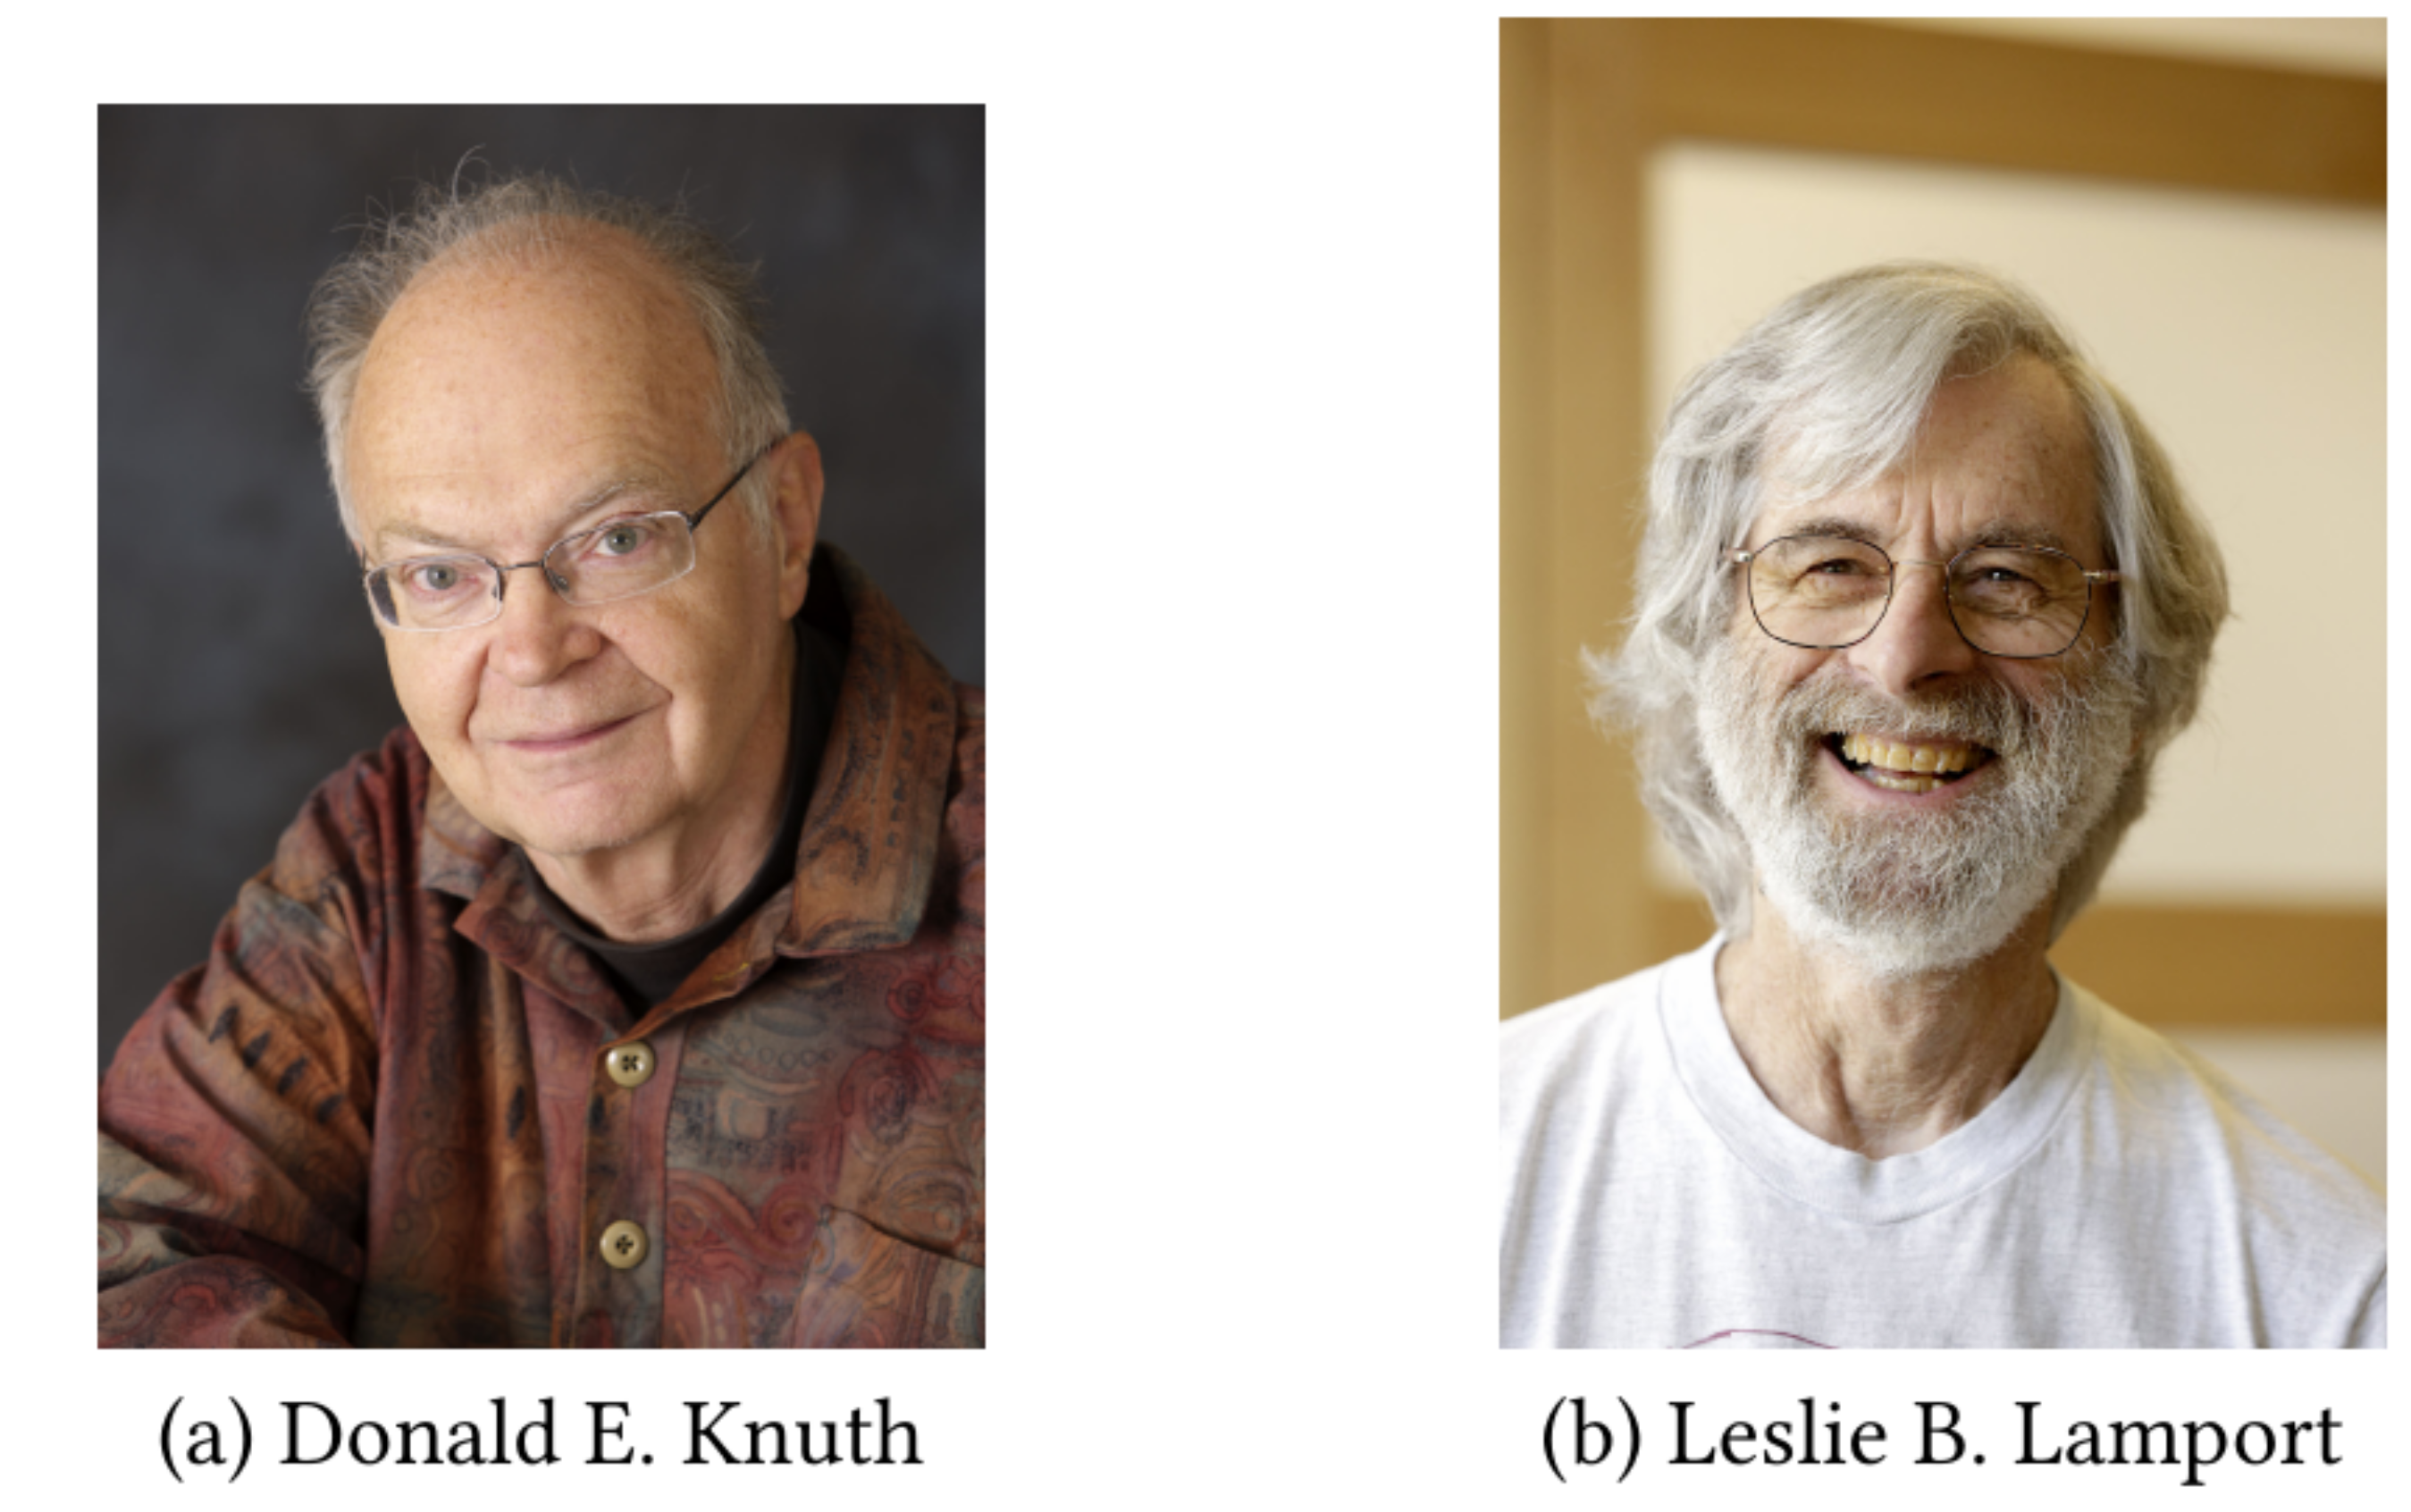
\includegraphics[width = 0.8\linewidth]{lamport-knuth}
  \caption{Os culpados!}
\end{figure}

\subsection{Mais e mais nomes: compiladores, interpretadores e formatos} %-----

Bom \ldots já sabemos que  \TeX{} e \LaTeX{} são coisas diferentes, entretanto,
interrelacionadas: o segundo é a forma mais utilizada, atualmente, para 
interagir com o primeiro.

Nesse ponto, seria interessante diferenciarmos \textit{engines} (motores/interpretadotes) 
de \textit{formats} (formatos).

O \TeX{} é um interpretador (\textit{engine}); o \LaTeX, um formato (\textit{format}).

\nota{
  Um outro formato que vimos é o \textit{Plain}~\TeX; e, atualmente, um formato 
  que se destaca é o \hrefA{https://en.wikipedia.org/wiki/ConTeXt}{\hologo{ConTeXt}}.
}

Os \textit{interpretadores} são os arquivos binários executáveis (ou seja, o 
programa em si); já os \textit{formatos} são macros (comandos ou instruções), 
baseadas em \TeX, que usamos para escrever nossos documentos (a grosso modo, são
linguagens ou atalhos para sequências de comandos ou estruturas em \TeX).

Não
\begin{marginfigure}
  \centering
  \href
  {
    https://www.lua.org/portugues.html
  }
  {
    
\includegraphics[width = 0.6\linewidth]{logo_lua.png}
  }
  \caption{Poderosa linguagem de programação (clique na imagem para saber mais)}
  \label{fig:lua}
\end{marginfigure}
é difícil perceber que o interpretador \TeX{} é bem antigo e que outros tenham
surgido ao longo desses anos.
De fato, à época do \TeX, nem existia ainda arquivos com extensão  \texttt{.pdf} 
-- a saída dos documentos era em DVI.
Quando surgiu o PDF, um interpretador ficou bem conhecido: \hologo{pdfTeX} -- cuja 
saída poderia ser em DVI que poderia ser convertida em PDF. 
O \hologo{pdfTeX} talvez seja o mais usado dentre os interpretadores que vamos 
falar, pois já vem selecionado, por padrão, em muitos editores dedicados ao 
\LaTeX \mn{%
  falaremos sobre editores para \LaTeX{} mais abaixo.}; 
as pessoas, simplesmente, não mudam a configuração padrão se realmente não 
for necessário.
Aliás, nosso sistema relaciona o \LaTeX{} com o \hologo{pdfTeX} usando um "atalho", 
denominado \hologo{pdfLaTeX}.

Portanto, o \hologo{pdfLaTeX} (que geralmente é o nome que aparecerá em nossos 
editores) é o \textit{interpretador} pdf\TeX\ com o \textit{formato} \LaTeX. 

Atualmente, dois interpretadores que se destacam são \hologo{XeTeX} e \hologo{LuaTeX}.
Além de serem mais rápidos, trazem implementações notáveis como seleção de fontes 
do próprio sistema (o \hologo{pdfTeX} não faz isso) ou interação com a linguagem 
de programação (brasileira) Lua (veja a Figura~\ref{fig:lua}). 
\nota{
  De acordo com Joseph Wright, usamos a palavra "compilação" herdada da computação,
  mas, uma palavra mais adequada seria "composição tipográfica" \cite{learnlatex}.
}
A saída de cada um deles é o PDF, diretamente.

Em nossos sistemas, ao usarmos \hologo{XeTeX} com \LaTeX{} usamos o atalho 
\hologo{XeLaTeX}.
Da mesma forma, \hologo{LuaTeX} com \LaTeX{} é simplificado por \hologo{LuaLaTeX}.

Obviamente, nesse minicurso, estamos interessados apenas no formato \LaTeX.
Também, por mera preferência, usaremos como interpretador o \hologo{LuaTeX}.
Portanto, "compilaremos" \, nossos arquivos com \texttt{lualatex}.

Obtamos por usar \lualatex, pois é o sucessor natural do \pdflatex. 
\sidenote{
  \footnotesize
  Confira essa informação no site \hrefB{http://www.luatex.org/}{http://www.luatex.org/}
}

\begin{atencao}{Mudanças à vista \ldots}{\exclamacao}
  Isso pode mudar algumas coisas para quem é acostumado a usar \pdflatex, 
  mas explicaremos as diferenças ao longo desse minicurso.  
\end{atencao}

Geralmente chamamos esses "atalhos" de \textbf{compiladores}
\mn{
  Para mais detalhes, veja \textcite{lualatex-doc}.
}.

Veja a Tabela~\ref{tab:compiladores} para comparação entre \textit{compiladores}, 
\textit{engine} e \textit{format}.

\begin{table}[!htbp]
  \centering
  \begin{tabular}{llc}
    \toprule
      \textbf{Compilador} & \textbf{Interpretador} & \textbf{Formato} \\
    \midrule
      \texttt{tex}           & \hologo{TeX}    & \hologo{plainTeX}       \\
      \texttt{pdftex}        & \hologo{pdfTeX} & \hologo{plainTeX}       \\
      \texttt{xetex}         & \hologo{XeTeX}  & \hologo{plainTeX}       \\
      \texttt{latex}         & \hologo{pdfTeX} & \LaTeX                  \\
      \texttt{pdflatex}      & \hologo{pdfTeX} & \LaTeX                  \\
      \texttt{xelatex}       & \hologo{XeTeX}  & \LaTeX                  \\
      \texttt{lualatex}      & \hologo{LuaTeX} & \LaTeX                  \\
      \texttt{texexec}       & \hologo{pdfTeX} & \hologo{ConTeXt}        \\
      \texttt{texexec --xtx} & \hologo{XeTeX}  & \hologo{ConTeXt}        \\
      \texttt{context}       & \hologo{LuaTeX} & \hologo{ConTeXt}        \\
    \bottomrule
  \end{tabular}
  \caption{Dando "nome aos bois"}
  \label{tab:compiladores}
\end{table}

Como 
\begin{marginfigure}
  \centering
  \href
  {
    http://www.luatex.org/
  }
  {
    
\includegraphics[width = 0.9 \linewidth]{logo_luatex.png}
  }
  \caption{
    Saiba mais sobre o \hologo{LuaTeX} acessando o link: 
    \href{http://www.luatex.org}{http://www.luatex.org}
  }
  \label{fig:lua}
\end{marginfigure}
esse texto é uma \sout{tentativa de} introdução ao \LaTeX, não chegaremos 
nem perto do que gostaríamos de expor sobre essa simbiose entre uma linguagem de 
\textit{programação} (Lua) integrada harmoniosamente com uma linguagem de 
\textit{marcação} (\LaTeX).
Basicamente, o código do \TeX{} foi reescrito em Lua (uma linguagem de programação
com muita relevância internacional, desenvolvida por brasileiros, na PUC-RJ), 
formando assim o \hologo{LuaTeX}.
Houve, intencionalmente, a projeção para que esse \textit{interpretador} fosse 
compatível com versões anteriores do \hologo{pdfTeX}, tornando o \hologo{LuaTeX} 
seu substituto natural, visto que é mais rápido e moderno.

Para encerramos essa subseção, é importante destacar a estabilidade do \LaTeX.
Basicamente temos duas versões: uma antes de 1993, a saber \LaTeX~2.09; e,
a de 1994 até HOJE, a saber \hologo{LaTeX2e}.
Isso é interessante, pois os códigos são praticamente preservados ao longo do 
tempo: você poderia rodar um código em \LaTeX\ de 20 anos atrás sem muitos 
problemas.

Todavia, quando falamos em \LaTeX{}, hoje, estamos nos referindo às 
funcionalidades trazidas na versão \hologo{LaTeX2e}.

\begin{marginfigure}
  \centering
  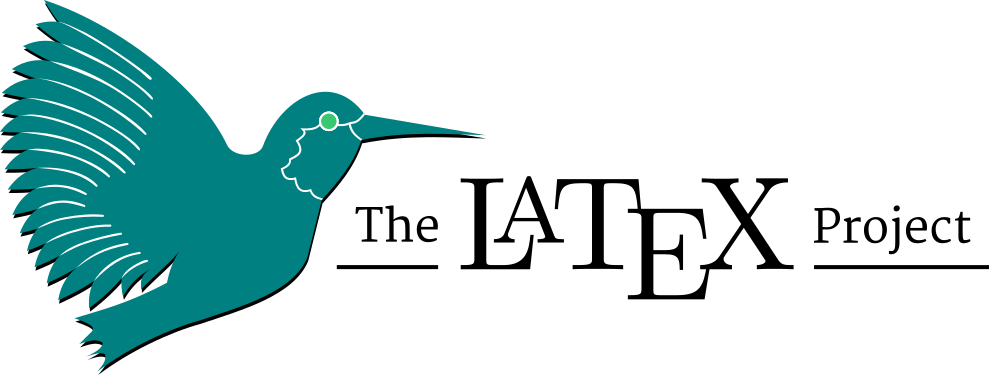
\includegraphics[width = \linewidth]{logo_latex}
  \caption{
    Saiba mais sobre esse fantástico projeto no link:
    \href{https://www.latex-project.org}{https://www.latex-project.org}
  }
  \label{fig:latexiii}
\end{marginfigure}

As atualizações são constantes, mas sem muitas mudanças estruturais.
Todavia, está em desenvolvimento uma terceira versão do \LaTeX, a saber, 
\hologo{LaTeX3} (veja a Figura~\ref{fig:latexiii}).

%------------------------------------------------------------------------------
\subsection{Como colocar o \hologo{LaTeX} em meu computador: as Distribuições}
%------------------------------------------------------------------------------ 

Para instalar localmente (em nosso computador) os \textit{interpretadotes}, 
precisamos das \textbf{distribuições}.

As principais são:

\begin{table}[!htbp]
  \centering
  \begin{tabular}{lll}
    \toprule
      \textbf{\sffamily Distribuições} & \textbf{\sffamily Sistema} & \textbf{\sffamily \textit{Download}/Instalação}\\
    \midrule
      \hologo{MiKTeX}   & Windows ou GNU/Linux ou Mac OS & \href{https://miktex.org/download}{https://miktex.org/download} \\ 
      \TeX{} Live       & GNU/Linux ou Windows           & \href{https://www.tug.org/texlive/acquire-netinstall.html}{https://www.tug.org/texlive/acquire-netinstall.html}\\
      Mac\TeX           & Mac OS                         & \href{https://www.tug.org/mactex/}{https://www.tug.org/mactex/}  \\
    \bottomrule
  \end{tabular}
\end{table}

A distribuição Mac\TeX{} contém todo o \TeX{} Live e adições específicas para 
Mac~OS.
\nota{
  Para GNU/Linux existem outras opções de instalação que economizam espaço.
  Tudo dependerá da necessidade de cada um:\\
  \texttt{texlive-latex-base}\\
  \texttt{texlive-latex-recommended}\\
  \texttt{texlive-pictures}\\
  \texttt{texlive-fonts-recommended}\\
  \texttt{texlive}\\
  \texttt{texlive-plain-generic}\\
  \texttt{texlive-latex-extra}\\
  Para mais informações veja essa discussão no \hrefA{https://tex.stackexchange.com/questions/245982/differences-between-texlive-packages-in-linux}{TeX SE}
}

O \TeX{} Live completo precisa de, aproximadamente, 5GB de espaço em disco.
Ele instala TODOS os pacotes disponíveis para \hologo{LaTeX}.
Como hoje em dia a capacidade de disco é relativamente grande, a instalação 
completa pode ser interessante, caso você não queira depender mais da internet 
para instalação de futuros pacotes.

Mas, se você quiser usar apenas o necessário e manter uma distribuição mínima em
seu computador, instalando futuros pacotes à medida que for precisando deles, 
talvez a distribuição \hologo{MiKTeX} seja a mais adequada.

\begin{atencao}{Atenção!}{\exclamacao}
  O processo de instalação depende do sistema operacioal e não será tratado nesse 
  texto, visto que usaremos distribuições ONLINE dos instrepretadores de \TeX{}.  
\end{atencao}

\section{Sim \ldots mas como eu uso?} %----------------------------------------
\label{sec:usando}

Certo \ldots já temos uma distribuição \TeX{}, e agora?
Basicamente, precisamos:

\begin{itemize}
  \item \textit{escrever}, usando o formato \hologo{LaTeX}, o que desejamos num 
    arquivo de texto com extensão \texttt{.tex};
  \item \textit{compilar}, ou seja, compor tipograficamente o arquivo \texttt{.tex}, 
    produzindo um arquivo \texttt{.pdf}; e, nesse ponto, usaremos o compilador 
    \texttt{lualatex};
  \item \textit{visualizar} o arquivo \texttt{.pdf}; nesse ponto, o visualizador
    de PDF é de escolha pessoal.
\end{itemize}

É uma boa prática salvar os arquivos \texttt{.tex} com nomes \textbf{sem acentuação}
ou \textbf{caracteres especiais} do teclado (\%, \$, *, etc.).
E, se o nome do arquivo for composto por mais de uma palavra, é aconselhável 
também \textbf{não deixar espaço entre elas}.

Por exemplo, suponha que você esteja escrevendo um artigo sobre \textit{números complexos}.
Seu arquivo principal não deve ser nomeado assim: 

\tcboxC{
  \texttt{Artigo! Números Complexos.tex}
}

Você deve retirar o \textit{ponto de exclamação} e o \textit{acento agudo}, bem 
como retirar os espaços entre as palavras.
Nesse último ponto, pode-se usar o \texttt{camelCase}, ou \texttt{snake\_case} 
ou separarar as \texttt{palavras-com-\textit{traço}}.
São aceitáveis qualquer das seguintes possibilidades (note que há uma preferência
por letras minúsculas):

%\begin{tcolorbox}
\tcboxC{
  \centering
  \begin{tabular}{l}
    \texttt{artigoNumerosComplexos.tex}\\
    \texttt{artigo-numeros-complexos.tex}\\
    \texttt{artigo\_numeros\_complexos.tex}\\
    \texttt{artigo\_numeros-complexos.tex}  
  \end{tabular}
}
%\end{tcolorbox}

Particularmente, prefiro essa última opção: onde se mistura o \textit{snake\_case}
com os traços.
Tento manter algum padrão antes do \textit{underline} e o nome do documento que 
estou escrevendo, separo por traços, caso seja necessário.
Essa abordagem pode ser interessante se você estiver trabalhando com um arquivo
principal (onde geralmente ocorre a compilação final) e muitos outros arquivos 
que serão incluídos no principal.

É uma forma de escrever \ldots
Há quem prefira escrever tudo em um único arquivo \texttt{.tex}!

Falaremos sobre manipulação de vários arquivos mais à frente, porém, apenas para
exemplificar a ideia, suponha que esse meu artigo (\texttt{artigo\_numeros-complexos.tex}) 
sobre números complexos seja composto de cinco seções:
\nota{
  Uma forma de nomear esses arquivos seria, respectivamente:\\
  \texttt{01\_intro-historica.tex}; \\
  \texttt{02\_representacoes.tex}; \\
  \texttt{03\_raizes.tex}; \\
  \texttt{04\_teo-fundamental.tex};\\
  \texttt{05\_conclusao.tex}.\\
  Notem que deixei a numeração no início, separando-a com \textit{underline} e 
  nomeei os arquivos de maneira que lembre-me a seção onde me encontro.
} 
introdução histórica; formas de representar um número complexo; raízes de um 
número complexo; o Teorema Fundamental da Álgebra; e, conclusões.
Então, desejamos escrever essas seções em arquivos separados e "incluí-los" no
arquivo principal, paulatinamente, por meio de compilações SOMENTE no arquivo
principal.

\begin{atencao}{Fica a dica!}{\exclamacao}
  Muitos nomeiam esses "arquivos principais", ou seja, onde ocorre a compilação, 
  de \texttt{main.tex} (ou \texttt{master.tex}), que significa, em inglês, 
  "principal", "importante", etc. ("senhor", "dominador", etc., para \textit{master}).
\end{atencao}

Para esse minicurso, à jato, começaremos com um arquivo principal, nomeado por
"\texttt{main.tex}", no qual escreveremos o conteúdo desejado inserindo as partes 
que o compõem, aos poucos.

\subsection{Como fazemos a "compilação"?} %------------------------------------

Bom \ldots ainda aprenderemos como escrever em \hologo{LaTeX}, não se preocupem,
mas, antes, vamos aprender como compomos tipograficamente o texto.

Já vimos que precisamos escrever o conteúdo do texto em um arquivo de extensão
\texttt{.tex} e compilarmos com \texttt{lualatex} \ldots 
Mas, como fazemos isso?

Ora, a escrita do texto pode ser feita em qualquer \textbf{editor de texto} de 
sua preferência.
Pode-se usar um "bloco de notas" (para usuários de Windows), ou o "evince" (para
usuários de GNU/Linux), por exemplo.
Apenas deve-se lembrar em salvar o arquivo com extensão \texttt{.tex}.

Também é aconselhável manter o arquivo \texttt{main.tex} em algum diretório (pasta) 
nomeado adequadamente.
Isso se deve ao fato de que, ao compilarmos, arquivos secundários são gerados (
.aux, .log, etc.), o qu epode gerar certa "bagunça".

Então, suponha que você tenha escrito um belo texto, cheio de equações matemáticas,
num arquivo denominado \texttt{main.tex}, salvo em um diretório por nome 
"\texttt{artigo\_tcc/}".
\begin{marginfigure}
  \centering
  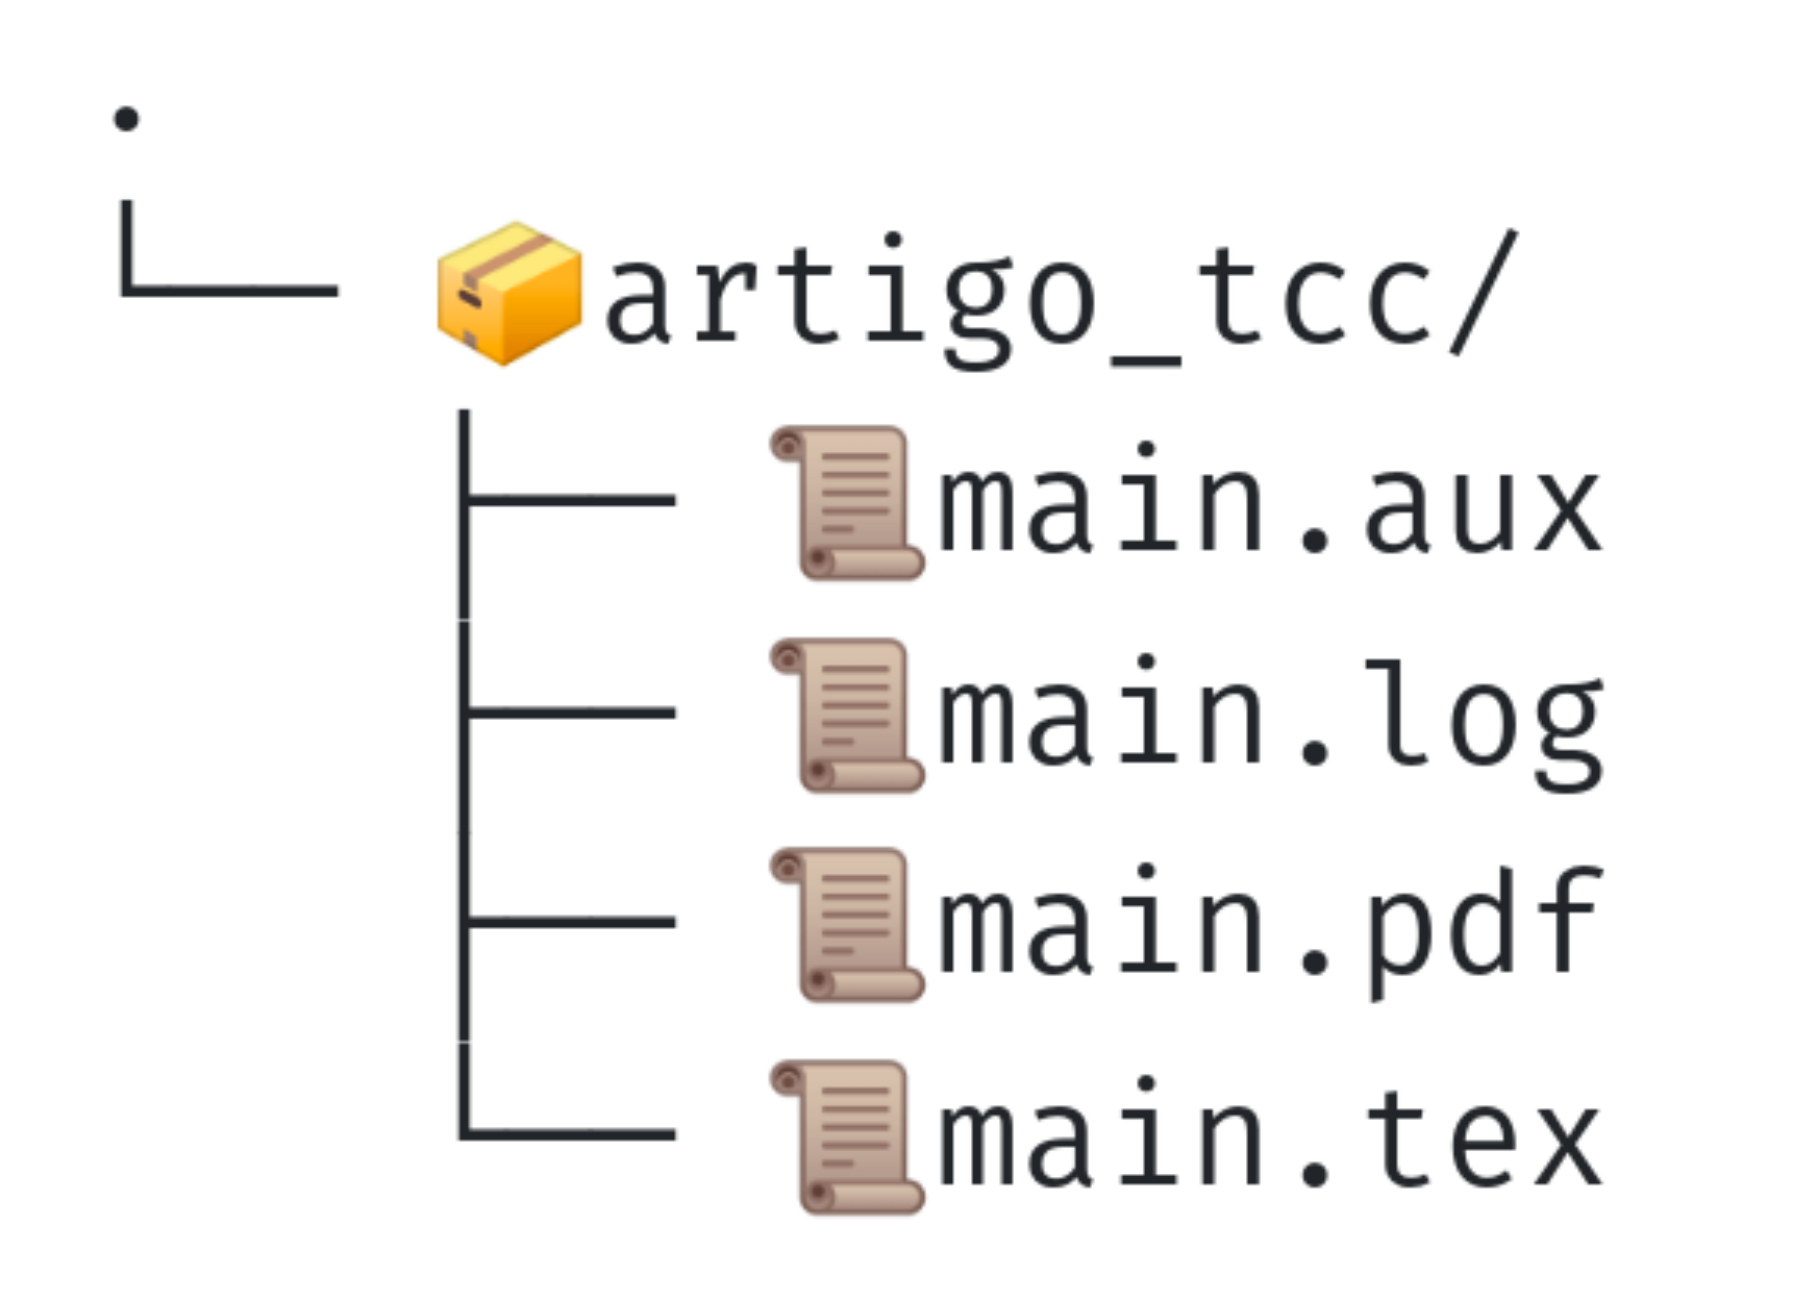
\includegraphics[width = 0.9\linewidth]{dir_lualatex.png}
  \caption{Arquivos gerados numa compilação simples}
\end{marginfigure}
Feito isso, abra o \textbf{terminal} (no Windows seria o "Prompt de Comando") 
dentro do diretório "\texttt{artigo\_tcc/}" e digite o seguinte comando:

\begin{codigo}{Usando o terminal para compilar}{\lapis}
  lualatex main.tex
\end{codigo}

Pelo menos três arquivos serão produzidos: um arquivo em \texttt[.pdf], que é a 
saída desejada; um arquivo \texttt{.aux}, essencial em referências cruzadas, por 
exemplo; e, um arquivo \texttt{.log}, o qual é um registro detalhado de tudo o que
ocorreu na compilação, inclusive possíveis erros.
Pode aparecer mais arquivos durante a compilação!
Tudo dependerá de quão complexo é seu texto (se possui sumário; index; lista de tabela;
lista de figura; glossário; etc).
A Tabela\ref{tab:aux} nos mostra alguns desses arquivos:

\begin{table}[!htbp]
  \centering
  \caption{Alguns dos possíveis arquivos gerados durante a compilação}  
  \label{tab:aux}
  \begin{tabular}{ll}
    \toprule
    \textbf{\sffamily Extensão} & \textbf{\sffamily Descrição}\\
    \midrule
    \texttt{.log} & registro detalhado sobre a compilação, inclusive erros \\
    \texttt{.aux} & registra processos intermediários, como referências cruzadas \\
    \texttt{.toc} & serve para produção do índice\\
    \texttt{.lof} & serve para produção da lista de figuras\\
    \texttt{.lot} & serve para produção da lista de tabelas\\
    \bottomrule
  \end{tabular}
\end{table}

Não tenha medo do terminal!
Ele é seu amigo!
Trabalhar usando "linha de comando", pelo terminal, é uma maneira de você 
comunicar-se com o computador de maneira rápida, direta e livre de distrações.
O comando \texttt{lualatex main.tex} simplesmente diz: "Olha \ldots componha
tipograficamente meu texto que está no arquivo \texttt{main.tex}, usando o 
interpretador \hologo{LuaTeX}, no formato \hologo{LaTeX}".

Mas, se você quiser mais funcionalidades na digitação (autocomplete, identação
automática, etc.) que um "bloco de texto" não oferece; bem como compilar sem 
usar o terminal, você precisará de um \textbf{editor de texto} especializado ou
uma IDE (\textit{Integrated Development Environment}).

\subsection{Editores para \LaTeX} %--------------------------------------------

\subsubsection{O \LaTeX\ é outro Word?} %--------------------------------------
\label{subsec:latex-word}

Um detalhe que precisamos ter em mente: a natureza dos editores para \LaTeX{}
é geralmente diferente dos editores de texto como \textit{Microsoft Word} ou 
\textit{LibreOffice Writer}.
Esses últimos editores são denominados WYSIWYG (acrônimo para a frase 
\textit{
  \textbf{W}hat \textbf{Y}ou \textbf{S}ee \textbf{I}s \textbf{W}hat \textbf{Y}ou \textbf{G}et
}).
\nota{
  "WYSIWYG \ldots O termo é usado para classificar ferramentas de edição e 
  desenvolvimento que permitem visualizar, em tempo real, exatamente aquilo que 
  será publicado ou impresso" (\hrefA{https://www.tecmundo.com.br/institucional/2057-o-que-e-wysiwyg-.htm}{TECMUNDO}, 
  acesso em 03/02/2022).\\
  Se você quiser saber como pronunciar corretamente essa sigla, acesse:
  \hrefA{https://youtu.be/GZuZxwIjh4I}{How to pronounce WYSIWYG}.
} 
Em uma tradução literal livre significa "O que você vê é o que você tem", ou 
seja, o que você vê na tela de seu editor, é o que aparecerá na impressão. 
No \LaTeX{} não é bem assim \ldots 
Você vê comandos misturados com texto normal, porém o resultado sairá diferente 
daquilo que estará vendo em seu editor! 
Ficará mais bonito o resultado, não se preocupe. =)

Poderíamos listar argumentos sobre a superioridade do \LaTeX{}, comparando-o ao 
\textit{Word} (por exemplo), mas isso não será feito. 
Cada um tem suas peculiaridades: vantajosas ou não. 
Tudo dependerá da finalidade do uso!
Particularmente, tenho encontrado no \LaTeX{} um ambiente próprio para escrita 
matemática de forma rápida, bonita e gratuita! 
Textos longos, cheios de capítulos, ou documentos personalizados --- como esse 
texto, exigiria um esforço e tempo tais, que nem passa por minha mente 
escrevê-los no Word (você já tentou criar um simples sumário no Word? 
Ou uma simples equação como esta: $\sum\limits_{n = 0}^{\infty} x^n = \frac{1}{1 - x}$, 
em menos de 10 segundos?)

Com isso em mente, é importante a aquisição de uma linguagem básica, mas, antes 
disso, vamos falar um pouco sobre os editores para \LaTeX.

\subsubsection{Indicações de editores para \LaTeX} %---------------------------

As possibilidades de editores são realmente vastas.
Portanto, comparar as funcionalidades dos principais editores é algo fundamental.
Você pode olhar uma comparação entre eles nesse link:

\begin{center}
  \textbf{
    \url{https://en.wikipedia.org/wiki/Comparison\_of\_TeX\_editors}
  }
\end{center}

Podemos usar editores \textbf{dedicados} ao \hologo{LaTeX} ou editores mais 
\textbf{genéricos}.

No que se refere aos editores dedicados, listamos:

\begin{table}[!h]
  \centering
  \begin{tabular}{ll}
    \toprule
    \multicolumn{1}{p{2cm}}{\centering\textbf{\sffamily Editor}}              & \multicolumn{1}{p{9.5cm}}{\centering\textbf{\sffamily Algumas características}}\\
    \midrule
      \hrefB{https://www.texstudio.org/}{\TeX studio}       & \multicolumn{1}{p{9.5cm}}{Destaca-se por ser multiplataforma e com muitos recursos.}\\
      \hrefB{https://www.texniccenter.org/}{\TeX nicCenter} & \multicolumn{1}{p{9.5cm}}{É voltado para usuários de Windows. Integra-se muito naturalmente ao sistema (e ainda indica o Sumatra para visualização do PDF).}\\
      \hrefB{https://www.lyx.org/}{LyX}                     & \multicolumn{1}{p{9.5cm}}{Esse é um editor diferente dos citados anteriormente; pois renderiza as equações e estruturas do texto de forma quase imediata. É o mais próximo, para \LaTeX, de editores WYSIWYG.}\\
    \bottomrule
  \end{tabular}
\end{table}

Agora, no que se refere aos editores mais genéricos, ou seja, não dedicados ao 
\LaTeX, mas que com o uso de \textit{plugins} essa realidade muda, destacam-se:

\begin{table}[!h]
  \centering
  \begin{tabular}{lcl}
    \toprule
      \textbf{\sffamily Editor} && \textbf{\textit{\sffamily Plugin}} \\
    \midrule
      \hrefA{https://www.gnu.org/software/emacs/emacs.html}{\sffamily GNU Emacs} && \href{https://www.gnu.org/software/auctex/}{\sffamily AUC \TeX}  \\                                       
      \hrefA{https://atom.io/}{\sffamily Atom}                                   && \href{https://atom.io/packages/atom-latex}{\sffamily atom-latex} \\
      \hrefA{https://neovim.io/}{\sffamily Neovim}                               && \href{https://github.com/lervag/vimtex}{\sffamily VimTeX}        \\
      \hrefA{https://code.visualstudio.com/}{\sffamily VSCode}                   && \href{https://marketplace.visualstudio.com/items?itemName=James-Yu.latex-workshop}{\sffamily \LaTeX\ Workshop}  \\  
    \bottomrule
  \end{tabular}  
\end{table}

Obviamente, para o iniciante, é indicado um editor dedicado ao \hologo{LaTeX}.
\sidenote{
  Particularmente, uso o VSCode com o \textit{plugin} do \LaTeX{} Workshop.
}

O \textit{plugin}  do \hologo{LaTeX} Workshop faz o processo de compilação de uma
forma um pouco diferente: ele usa uma ferramenta chamada \textbf{latexmk} que 
nada mais é que um \textit{script} que automatiza muitos processos.
Por exemplo, quando o documento é complexo; com referências cruzadas; sumário; 
glossário; lista de tabelas; lista de figuras; etc. é necessário mais de um processo
de compilação. 
Esse \textit{plugin} faz isso tudo parecer mágica.
Ele vem, por padrão, configurado para \pdflatex, mas pode ser modificado
o interpretador de maneira bem simples.

Uma ferramenta parecida com o \texttt{latexmk}, mas que precisa de diretivas (
você precisa "dizer" para ele os passos que deseja executar) é o \textbf{arara}.
Ele foi desenvolvido por um brasileiro (Paulo Cereda) e possui ferramentas de 
\begin{marginfigure}
  \centering
  \href
  {
    https://gitlab.com/islandoftex/arara
  }
  {
    
\includegraphics[width = \linewidth]{logo_arara.pdf}
  }
\end{marginfigure}
limpeza de arquivos auxiliares; rapidez na segunda compilação; produção de arquivo 
\textit{draft} (um rascunho que não gera o conteúdo pdf, mas apenas verifica a 
sintaxe do documento -- o que torna as coisas muito mais rápidas); etc.
Falaremos sobre ele no Apêndice~\ref{apend-A:arara}, pois vale muito a pena 
conhecer essa ferramenta!

\section{Overleaf: um editor \textit{online} notável} %------------------
\label{sec:overleaf}

Como nosso minicurso é \textit{online} e possui tão curto tempo, não seria 
possível um auxílio na instalação de uma distribuição \TeX{}, editor dedicado, 
nem tampouco um visualizador de PDF de cada um de vocês, localmente.

Usaremos, então, uma plataforma que reúne tudo isso de forma \textit{online} e 
gratuita (para aquilo que desejamos): \Overleaf.
\nota{
  Exitem outros editores online que poderíamos usar:
  \hrefA{https://papeeria.com/}{Papeeria} ou
  \hrefA{https://www.authorea.com/}{Authorea}, por exemplo.
}
Vamos conhecer alguns recursos disponíveis do \Overleaf, antes de iniciarmos a
aquisição da linguagem \hologo{LaTeX}.

O primeiro passo é acessar o \textit{link} e fazer um registro (\textit{Register}) 
de uma conta (é possível fazer o \textit{login} com uma conta Google), logando na
plataforma \textit{online} (Veja Figura~\ref{fig:overleaf_inicio}):

\begin{figure}[!htbp]
  \centering
  \href
  {
    https://www.overleaf.com/
  }
  {
    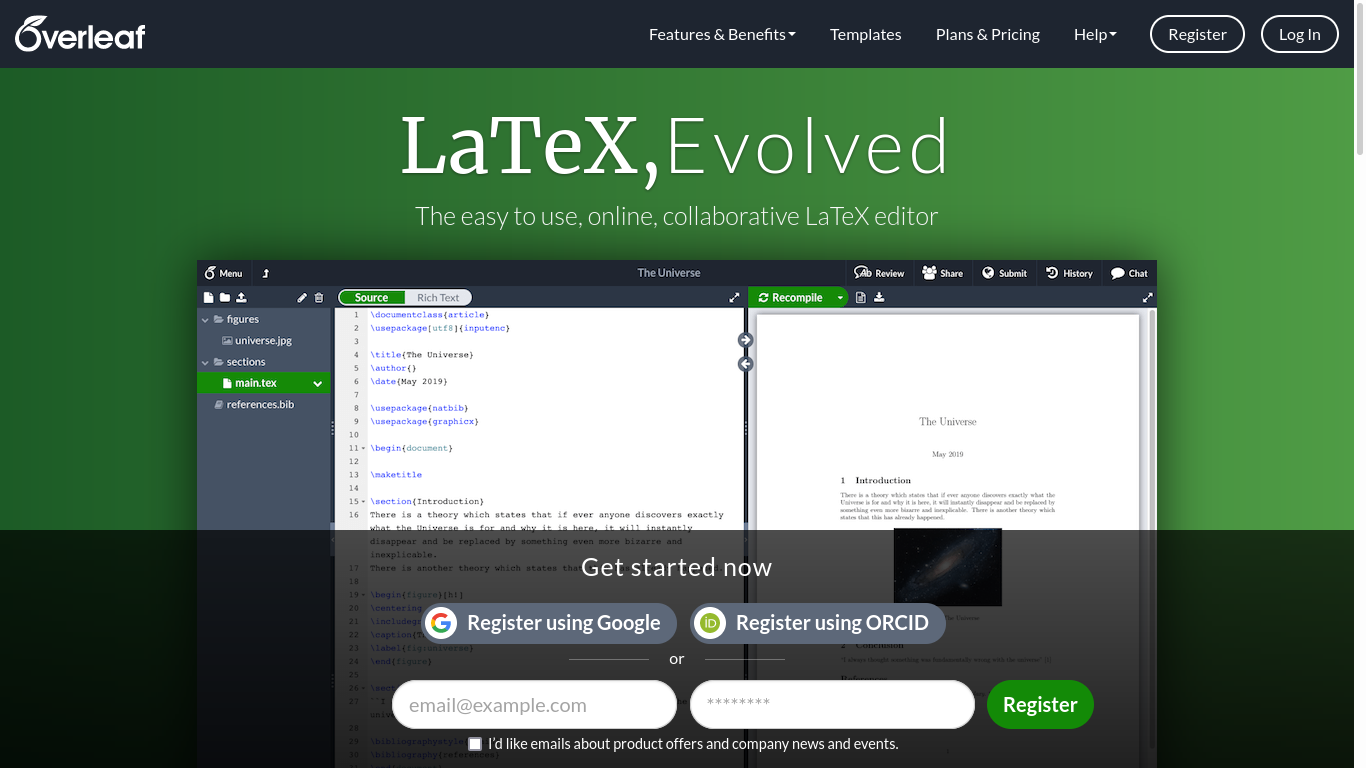
\includegraphics[width = 0.8\linewidth]{overleaf_inicio}
  }
  \caption{\url{https://www.overleaf.com/}}
  \label{fig:overleaf_inicio}
\end{figure}

Ao entrar no \Overleaf, aparecrá uma tela como é mostrado na Figura~\ref{fig:overleaf_panorama-EN}

\begin{figure}[!h]
  \centering
  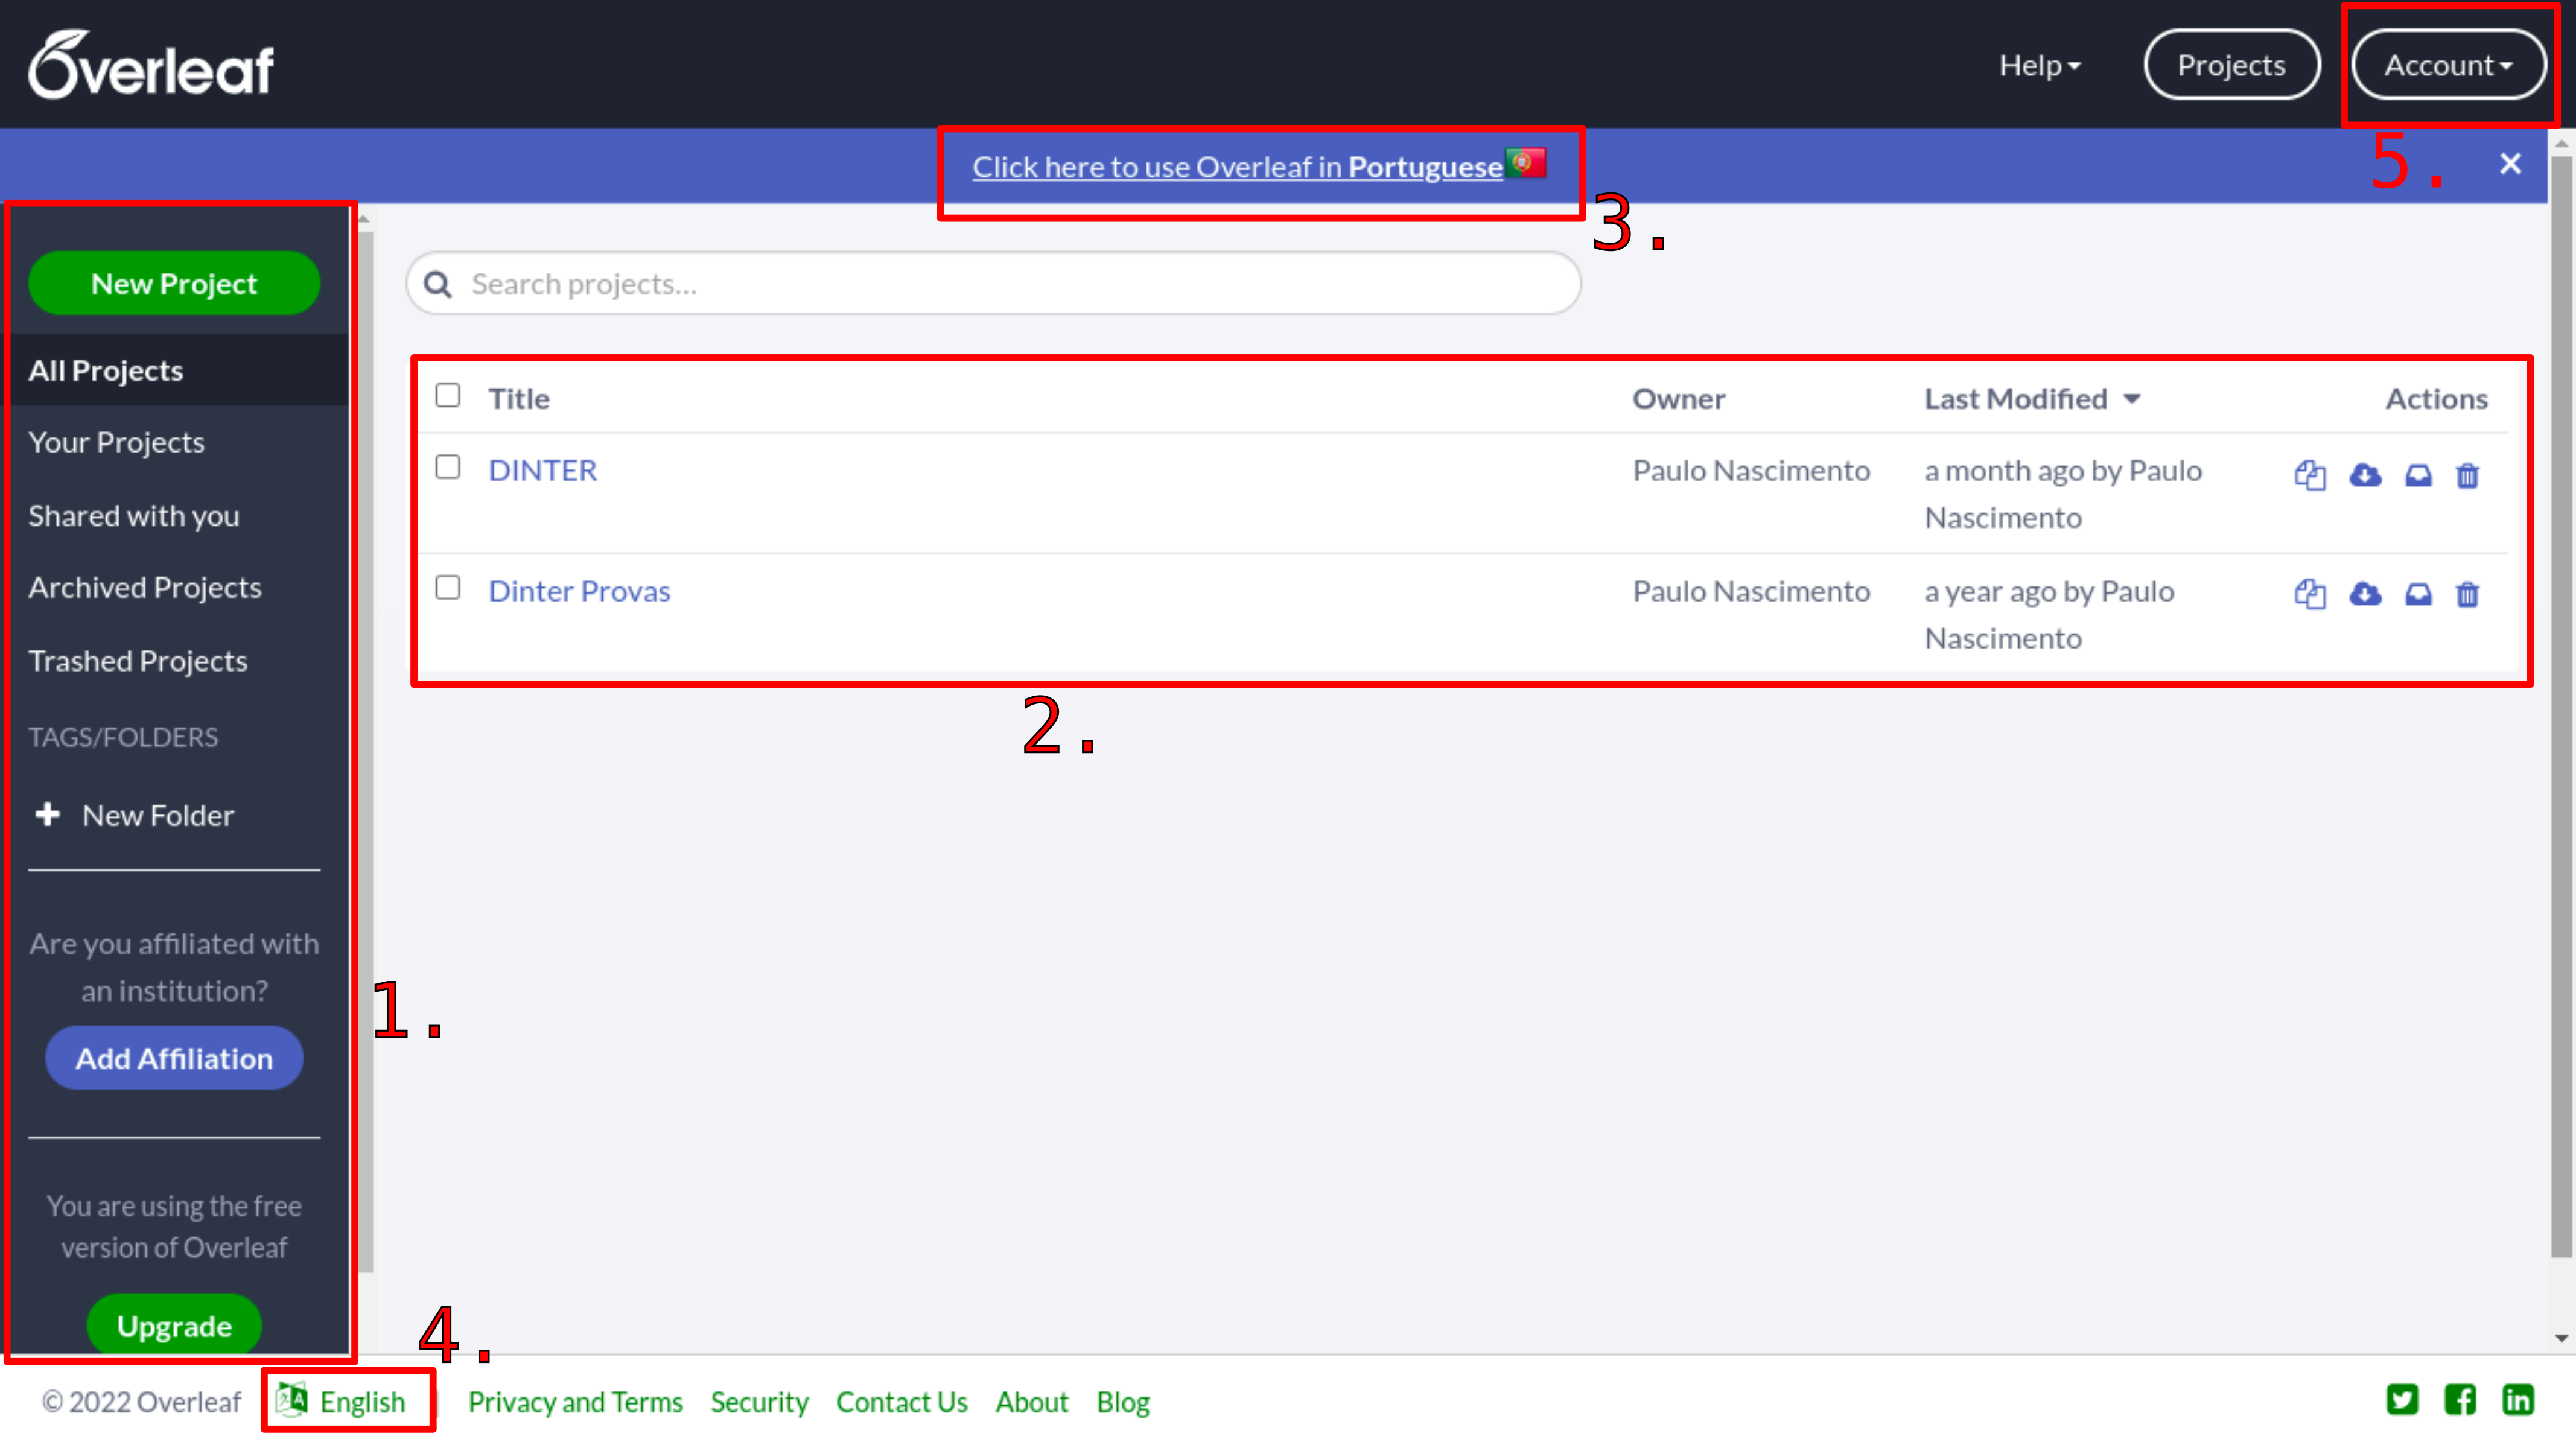
\includegraphics[width = 0.8\linewidth]{overleaf_panorama-EN}
  \caption{Visão inicial do Overleaf}
  \label{fig:overleaf_panorama-EN}
\end{figure}

Vamos explicar o que significa cada nicho destacado:

\begin{enumerate}
  \item Aqui é onde iniciaremos um \textbf{Novo Projeto} (\textit{New project}),
        que poderá ser em Branco; ou de algum modelo que o próprio \Overleaf{} 
        disponibiliza; ou do GitHub; etc.;
  \item Nesse nicho aparecerão todos os seus projetos (no meu caso, tenho 2 em 
        andamento);
  \item Você pode modificar o idioma por aqui;
  \item Também é possível fazermos a modificação do idioma por aqui;
  \item Você pode sair do \Overleaf{} clicando nesse botão e, em seguida, 
        \textsf{Sair} (\textit{LogOut})
\end{enumerate}

Escolha o item "3" ou "4" para modificar o idioma para \textsf{Portugues}.
Em seguida, abra um projeto em branco, seguindo o caminho:

\begin{center}
  \textsf{Novo Projeto} $\quad \longrightarrow \quad$ \textsf{Projeto em Branco}
\end{center}

Aparecerá uma janela para que você coloque o título do projeto.
Escreva:

\tcboxC{\sffamily \bfseries minicurso-EMAT\_LaTeX}

Entraremos naquilo que vamos denominar {\sffamily Área de Trabalho do Overleaf}
(algo como a Figura~\ref{fig:overleaf_desktop}).

\begin{figure}[!htbp]
  \centering
  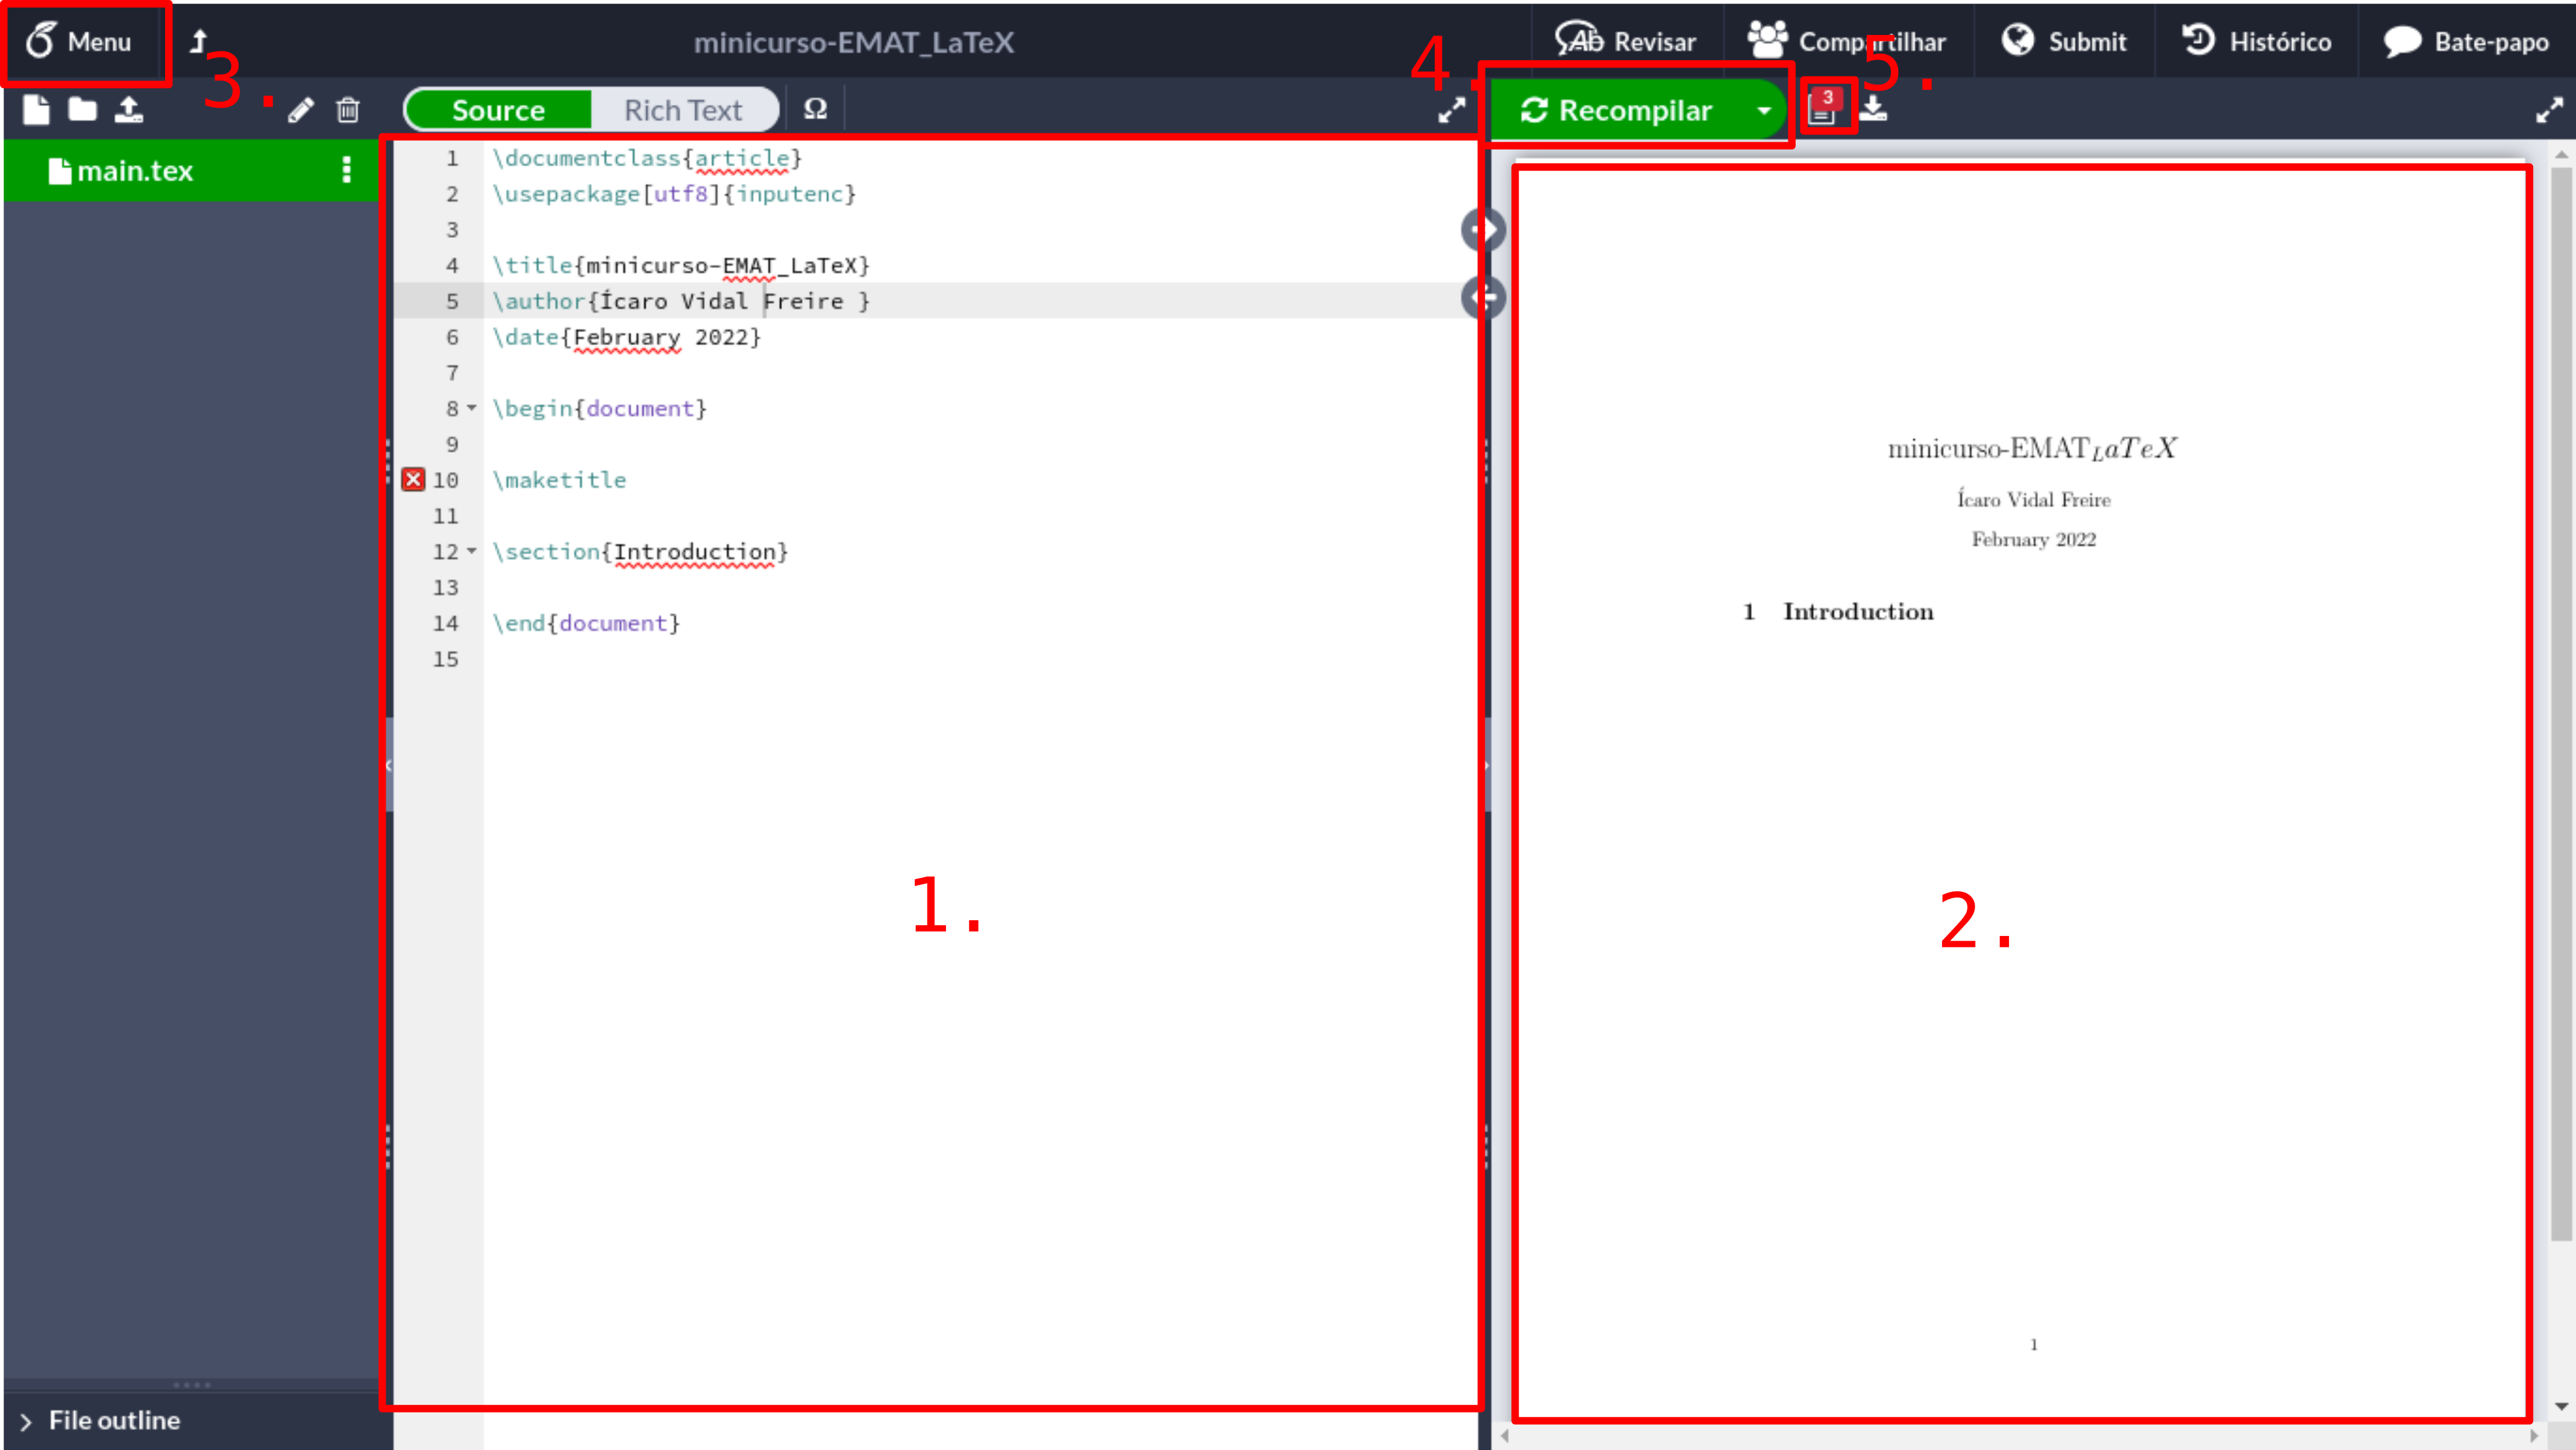
\includegraphics[width = 0.9\linewidth]{overleaf_area-trabalho}
  \caption{Visão da Área de Trabalho dos Projetos, no Overleaf}
  \label{fig:overleaf_desktop}
\end{figure}

Vamos modificar o compilador (lembrem-se que usaremos o \lualatex, não o 
\pdflatex{} -- que é o padrão do \Overleaf), mas, antes, vamos connhecer 
um pouco essa área de trabalho:

\begin{enumerate}
  \item Digitamos os códigos nesse espaço! 
        Aqui é onde escreveremos a lingugem do \hologo{LaTeX}.
        Notem que o \Overleaf{} já usou o seu nome e o nome do projeto para 
        preencher algumas coisas nessa linguagem;
  \item A saída do \texttt{pdf} é mostrada aqui.
        A renderização é automática, o que facilita muito o aprendizado para 
        iniciantes;
  \item Nesse espaço modificamos muita coisa no \Overleaf{}, especificamente, 
        modificamos algumas congigurações, inclusive o \textsf{compilador}.
        Também podemos fazer o \textit{download} do PDF ou do Código por aqui.
  \item No botão \textit{Recompile} existem muitas opções para renderizar o 
        documento.
  \item É aqui que você pode configurar para compilação automática; ou produzir
        um documento \textit{draft} (rascunho); ou para checagem das sintaxes;
  \item Por fim, aqui mostra mensagens de erros ou alertas. 
        Inclusive, há três mensagens de erros por lá! 
        Veremos que a mensagem, na realidade, resume-se a um único problema: 
        Ao aproveitar o título de nosso projeto e escrevê-lo no título do 
        documento, o \Overleaf{} usou um \textbf{caractere especial} no modo 
        \textsf{Texto}, mas que é exclusivamente reservado ao 
        \textsf{Modo Matemático} \emoji{man-shrugging-light-skin-tone}.
\end{enumerate}

\begin{atencao}{Atenção!}{\exclamacao}
  Em \textsf{Menu} (ver item 3 da Figura~\ref{fig:overleaf_desktop}), altere o
  compilador modificando na seção \textit{Settings}, item \textit{Compiler}, de
  \textsf{pdfLaTeX} para \textsf{LuaLaTeX}.
\end{atencao}

O nosso fluxo de trabalho será:

\begin{enumerate}[\ding{226}]
  \item \textbf{\textsf{escrever}} o texto e os códigos na área adequada;
  \item \textbf{\textsf{compilar}} (compor tipograficamente) o documento;
  \item \textbf{\textsf{depurar}} possíveis erros;
  \item \textbf{\textsf{admirar}} o resultado \emoji{relieved-face}.
\end{enumerate}

Algumas outras peculiaridades do \Overleaf{} veremos quando estivermos praticando
a linguagem do \LaTeX{} nos exercíos!
Então, agora, resta-nos aprender os rudimentos dessa linguagem.

\newpage
%
  \part{Aprendendo a Linguagem LaTeX}
%
    \section{Uma Linguagem} %------------------------------------------------------
\label{sec:aprendendo}

\begin{margintable}\vspace{.8in}\footnotesize
  \caption{Sumário da \textsc{Part II}}
  \medskip
  \begin{tabularx}{\marginparwidth}{|X}
    \textbf{\sffamily \textcolor{azulUFRB}{Seção}~\ref{sec:aprendendo}}.    {\sffamily Uma Linguagem} \\
  \end{tabularx}
\end{margintable}

A aquisição de uma linguagem não é algo imediato (para a maioria das pessoas); e,
o \LaTeX{} é uma linguagem, conhecida como \textit{linguagem de marcação}.
Isso implica que há uma \textsf{estrutura} e \textsf{simbologia} características, 
ou seja, é necessário um investimento em tempo e esforço para uma certa fluidez 
na comunicação ou escrita.

Vimos na Subseção~\ref{subsec:latex-word} que o \hologo{LaTeX} é uma linguagem 
que envolve \textit{códigos} e \textit{texto}.
Sua estruturação é diferente de sistemas \textsf{WYSYWYG} (como o Word) e, à
primeira vista, demanda um ``esforço técnico'' maior no início do aprendizado, 
mesmo para documentos simples.
Mas, à medida que a complexidade do documento aumenta, o esforço empregado ao 
usar o \LaTeX{} é menor, quando comparado à sistemas \textsf{WYSYWYG}, para 
produzir o mesmo documento.
A Figura~\ref{fig:latex-vs-word} mostra um vislumbre dessa ideia, embora seja
apenas hipotética.

\begin{figure}[!htbp]
  \centering
  \caption{Complexidade do Documento vs Esforço empregado}
  \label{fig:latex-vs-word}
  \medskip
  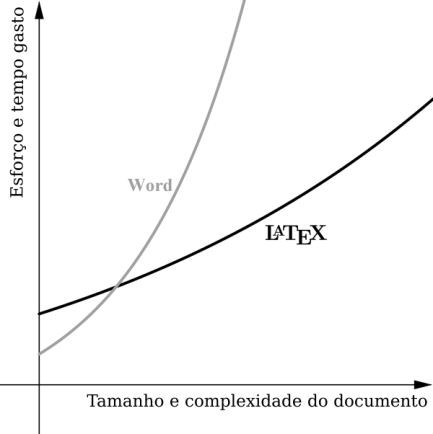
\includegraphics[width = 0.6\linewidth]{figs/latex-vs-word.png}
  
  {\small \textsf{Fonte:} \url{https://latexcfp.wordpress.com/}}
\end{figure}

\begin{marginfigure}
  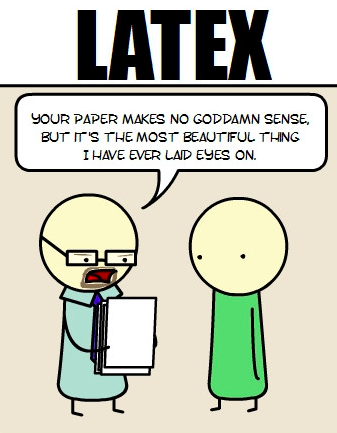
\includegraphics[width = \linewidth]{piada-latex.png}
  
  {
    \sffamily
    \textit{Seu artigo não faz nehum sentido para 
    mim, mas é a coisa mais linda que eu já vi!}
    (Tradução livre e suavizada \emoji{grinning-face-with-sweat})
  }
  
  {\textsf{\textbf{Fonte:}} \href{http://nvisnjic.com/2015/01/13/mathjax-magic.html}{The magic of LaTeX.}}
\end{marginfigure}

Além disso, é notável a beleza da composição tipográfica final, em especial (mas
não necessariamente) quando o documento envolve equações matemáticas.
Como vimos, essa \textsf{beleza} é fruto das mais sofisticadas técnicas empregadas 
nos algorítimos que produzem a saída \texttt{0} ou \texttt{1}, representando, 
respectivamente, ``sem tinta'' ou ``com tinta''.

\subsection{Um pouco sobre a estruturação do LaTeX} %--------------------------

Antes de aprendermos os símbolos pertinentes dessa linguagem, é interessante 
conhecermos um pouco de sua estruturação.
% 
  \subsubsection{Comandos}
% 
Um comando no \LaTeX{} sempre começa com uma barra invertida (``\textbackslash'').
Tal comando pode está inserido em \textsf{modo texto} ou em \textsf{modo matemático}.\mn{
  Existe toda uma sintaxe para o \textsf{modo matemático}, que vamos deixar para
  abordar em outra seção.
}
Por exemplo, quando escrevemos \verb|\LaTeX|, com o ``L'', ``T'' e ``X'' maiúsculos, 
o resultado depois da compilação é: \LaTeX.
Mas, se digitarmos \verb|\Latex|, uma mensagem de erro será mostrada, visto que 
esse comando não vem por padrão definido.

Tal exemplo já nos mostra uma outra característica da estruturação da linguagem 
que estamos conhecendo: ela é \textit{case sensitive}, ou seja, é sensível à
letras maiúsculas e minúsculas.
O comando \verb|\LaTeX| é difernete do comando \verb|\latex|, que é diferente do
comando \verb|\Latex|.
\mn{
  \texttt{\textbackslash LaTeX} $\neq$ \texttt{\textbackslash Latex} $\neq$ \texttt{\textbackslash latex}
}

\begin{atencao}{Atenção!}{\exclamacao}
  Inclusive, essa é uma das grandes fontes de erro de quem está começando no 
  \LaTeX: a digitação de um comando de forma errada é muito comum!
\end{atencao}

Também é importante ressaltar que comandos podem vir acompanhados de 
\textbf{\textsf{argumentos obrigatórios}}, que colocamos entre \textsf{chaves} 
(``\texttt{\{\ldots\}}''); ou de \textbf{\textsf{argumentos opcionais}}, que colacamos 
entre \textsf{colchetes} (``\texttt{[\ldots]}'').

Por exemeplo, o comando \verb|\documentclass| define a \textsf{classe} do 
documento.
O argumento da classe é obrigatório, ou seja, precisamos ``indicar'' ao \LaTeX{}
se estamos usando um \textsf{artigo} (\textit{article}); um \textsf{livro} 
(\textit{book}); um relatório (\textit{report}); uma apresentação (\textit{beamer});
etc.
Além disso, existem vários argumentos opcionais, dentre os quais descato: o 
tamanho da fonte, que por padrão é \texttt{10pt}\mn{ 
  são três opções possíveis nas classes \textit{standard}: \texttt{10pt}, 
  \texttt{11pt} e \texttt{12pt}.
}
; o formato do papel, por exemplo, \texttt{A4}; e a opção de \textit{layout} para
estruturar as margens à impressão em frente e verso: \texttt{twoside}.
Veja como ficaria o comando para a classe \texttt{article}; com tamanho da fonte 
de \texttt{12pt}; definida para um formato de paper \texttt{A4}; e, com a opção 
de imprimir em frente e verso:\mn{
  Note que o comando opcional \texttt{twoside} não ``diz'' para a sua impressora 
  imprimir em ``frente e verso''.
  Apenas configura as margens das páginas para essa opção.
}

\tcboxC{
  \ttfamily \textbackslash documentclass[12pt, a4paper, twoside]\{article\}
}
% 
  \subsubsection{Classe do Documento}
% 
Notem que uma \textsf{classe} possui características instrínsecas: um artigo 
não possui capítulos, mas seções; o que é diferente de um livro, que possui 
essas duas estruturas, por exemplo.
Existem \textsf{classes} que já vem, por padrão, nas distribuições \TeX{} que 
conhecemos e inúmeras outras implementadas pela comunidade de usuários do \LaTeX.

A Tabela~\ref{tab:classes-nativas}, mostra algumas dessas \textsf{classes} 
\textsf{nativas} (também chamadas de \textsf{padrão} ou \textit{standard}).

\begin{margintable}
  \centering
  \caption{Algumas das \textsf{classes} \textit{standard} do \LaTeX}
  \label{tab:classes-nativas}
  \begin{tabular}{lcl}
    \toprule
      \textbs{Classe}  && \textbs{Finalidade} \\
    \midrule
      \textit{article} && artigo     \\
      \textit{book}    && livros     \\
      \textit{report}  && relatórios \\
      \textit{letter}  && carta      \\
    \bottomrule  
  \end{tabular}  
\end{margintable}

\begin{atencao}{Atenção!}{\exclamacao}
  Por conta da limitação de nosso tempo, vamos tangenciar alguns aspectos da 
  linguagem \hologo{LaTeX}, usando apenas a classe \textit{article}.
\end{atencao}

Você já deve ter imaginado que existe uma infinidade de \textsf{classes} para o
\LaTeX, além das nativas.
De fato, há uma comunidade ativa que contribui com seus talentos e disponibilizam,
em sua grande maioria, de forma gratuita muitas funcionalidades/ferramentas que 
facilitam a vida de usuários do \LaTeX.
Dentre essas funcionalidades/ferramentas, estão as \textsf{classes}.
Mas, existem \textbf{pacotes}; aplicativos em java (como o \textsf{arara}); etc.
Geralmente, as \textsf{classes} modificam a estrutura geral de um documento.
Como vimos, um \textsf{artigo} possui uma estrutura diferente de um \textsf{livro},
por exemplo.
O que define essas estruturas são as \textsf{classes}.\en{%
  A extensão do arquivo para uma classe é \texttt{.cls}
}

\begin{atencao}{Atenção!}{\exclamacao}
  Cada classe possui sua sintaxe específica para alguns comandos, porém alguns 
  outros comandos são gerais e servem para a maior parte das classes. 
  Estudaremos apenas esses últimos.
  Caso você queira trabalhar com uma classe diferente da “nativa”, deve 
  verificar o manual para os detalhes.
\end{atencao}

Dentre as classes que não são nativas ao \hologo{LaTeX}, gostaria de destacar:
\nota{
  É bem engraçada, e realista, a descrição do nome abn\TeX:\\ 
  {
    \centering \textit{ABsurd Norms for TeX}.\\
  }
  Por que será, né? \emoji{hand-over-mouth}
}

\begin{description}
  \item[\textas{abn\TeX 2}] Se você pensa em escrever seu Trabalho de Conslusão 
                   de Curso, usandoo \LaTeX, você precisa ler a documentação e 
                   conhecer bem essa classe.
                   Ela, basicamente, fornece um modelo canônico (\textit{template})
                   para várias estruturas de cunho científico, dentro do padrão 
                   da \textsc{abnt} (Associação Brasileira de Normas Técnicas).
                   Você não precisará se preocupar com as configurações de todas
                   aquelas normas em seu texto!
                   Conhecendo os comandos da classe, você só se preocupará com 
                   o \textsf{conteúdo}, não com a \textsf{estrutura}.
                   Inclusive, estou desenvolvendo uma clase para monografia do 
                   curso de Licenciatura em Matemática da UFRB, baseada na classe
                   abn\TeX 2.
                   Ela está disponível lo \textit{link}: 
                   \hrefB{https://github.com/icaro-freire/tccUFRB}{\textsf{tccUFRB.cls}}
  \item[\textas{beamer}] Esta é uma classe para apresentações em \textit{slides} 
                   (chamado também de \textit{frame}, pelos usuários).
                   A qualidade das apresentações é surpreendente. 
                   Principalmente quando a apresentação envolve fórmulas 
                   matemáticas (não distorce como acontece por aí \ldots)!
                   Existem uma infinidade de \textit{templates} (oficiais ou não) 
                   disponíveis que você, certamente, encontrará um que atenda às 
                   suas necessidades.
                   O manual do \textsf{beamer} pode ser visto no \textit{link}:
                   \hrefB
                   {
                     http://tug.ctan.org/macros/latex/contrib/beamer/doc/beameruserguide.pdf
                   }
                   {
                     The \textsc{beamer} \textit{class}
                   }
                   \newline
                   Um \textit{template} de tema claro, extra oficial, que 
                   recomendo para \textsf{beamer} é o 
                   \hrefB{https://github.com/matze/mtheme}{Metropolis};
                   e, um escuro (\textit{dark}): 
                   \hrefB{https://github.com/junwei-wang/beamerthemeNord}{The Nord Beamer Theme.} \\
                   Um pequeno manual, em espanhol, que considero muito prático e 
                   eficiente (principalmente se você não quiser ler as 234~p do 
                   manual oficial) é: 
                   \hrefB{http://metodos.fam.cie.uva.es/~latex/apuntes/apuntes13.pdf}{Presentaciones en \LaTeX\ con Beamer.}
  \item[\textas{exam}] Essa é uma classe para confecção de listas de atividade.
                   Possui um ambiente para soluções; comandos para pontuação nas
                   questões; cria cabeçalhos e rodapés estilizados; etc.
                   Se você é professor e usa fórmulas em suas listas de 
                   atividades, recomendo fortemente ler a documentação dessa 
                   classe \textsf{exam.cls}.
                   Você encontrará o manual nesse \textit{link}:
                   \hrefB{https://ctan.dcc.uchile.cl/macros/latex/contrib/exam/examdoc.pdf}{Using the exam document class}.
                   \newline
                   Baseada nessa classe, desenvolvi (e estou no processo de 
                   atualização) a classe \hrefB{https://github.com/icaro-freire/ativmatUFRB}{ativmatUFRB.cls}.
                   Ela é uma classe não oficial para listas de atividades do 
                   curso de Licenciatura em Matemática, da UFRB.
                   Possui um cabeçalho estilizado com o logo da universidade, bem
                   como comandos e informações que considero úteis num documento
                   desse tipo.
\end{description}

% 
  \subsubsection{Mais sobre Comandos}
% 

Uma pergunta que talvez possa surgir nesse momento: 
\textit{
  se cada comando começa com a ``barra invertida'', qual o comando para 
  representar a própria barra invertida? 
}
  \emoji{thinking}\\
É natural pensarmos em ``\textbackslash\textbackslash'', mas a pergunta surgiria 
novamente: 
\textit{ 
  como representar ``\textbackslash\textbackslash''?
} \emoji{exploding-head}\\
E seguiria uma sequência infinita de pergutas, não?!

Bom, para que essas questões possam ser resolvidas, você deve ter em mente que 
alguns símbolos são \textsf{reservados}, ou seja, há um conjunto de definições 
internas ao próprio \LaTeX. 
Inclusive, símbolos usados em estruturas internas de comandos. 
É o caso de ``\textbackslash'': ele é usado para iniciar qualquer comando no \LaTeX. 
Se você quiser representá-lo textualmente, pode usar \texttt{\textbackslash textbackslash}.
\en{ 
  Veremos que, no modo Matemático, esse mesmo comando pode ser representado 
  simplesmente por \texttt{\textbackslash backslash}.
}

A Tabela~\ref{tab:especial} mostra alguns desses caracteres especiais. 
\begin{table}[!htbp]
  \caption{Caracteres Especiais no \LaTeX}
  \label{tab:especial}
  \centering
  \begin{tabular}{ccl}
    \toprule
      \textbs{Caractere}      && \textbs{Descrição} \\
    \midrule
     \texttt{\textbackslash}  && inicia um comando                                  \\
      \texttt{\%}             && para comentar código                               \\ 
      \texttt{\~{}}           && evita separação de palavras                        \\
      \texttt{\{\;\}}         && delimita códigos                                   \\
      \texttt{\&}             && separa colunas numa tabela                         \\
      \texttt{\#}             && exibe $\textrm{n}^\circ$ de parâmetros num comando \\
      \texttt{\$}             && usado no modo matemático                           \\
      \texttt{\^{}}           && usado para potências                               \\ 
      \texttt{\_{}}           && usado para subíndices                              \\
    \bottomrule
  \end{tabular}
\end{table}

Se você quiser exibir qualquer um deles, (excetuando a \textit{barra invertida},
claro) basta colocar a barra invertida antes dos símbolos!
Por exemplo, se deseja exibir ``10\%'', deve digitar: \texttt{10\textbackslash \%}.

Ainda falando sobre comandos \ldots\ se você for utilizar algum comando interno, 
ou mesmo algum criado por você (sim isso é possível, mas não veremos nesse 
microcurso \emoji{confused-face}), deve ter um cuidado especial com o espaçamento 
de alguma palavra depois do referido comando.
Por exemplo, se formos escrever 
\tcboxC{O \LaTeX\ é sensacional!}
\textbf{não} devemos fazer ``\texttt{O \LaTeX\ é sensacional!}'', visto que a 
saída produzida por esse último comando é:
\tcboxC{O \LaTeX é sensacional!}
Devemos, portanto, colcar ``\texttt{\{\}}'' ou ``\texttt{\textbackslash}'' 
ao final do comando. 
Isso faz com que haja um pequeno espaço entre ele e a próxima palavra. 
Em resumo, você deve fazer alguma das seguintes maneiras:
\begin{enumerate}
  \item[(i)] \texttt{O \textbackslash LaTeX\{\} é sensacional!}
  \item[(ii)] \texttt{O \textbackslash LaTeX\textbackslash\ é sensacional!} 
\end{enumerate}

Gostaria de destacar o uso do comando \texttt{\%} para comentários de código! 
Use-o sempre para lembrar-se de algo ou para organização. 
Ao longo desse texto, esse comando será usado constantemente.

% 
  \subsubsection{Ambientes}
% 

Um agrupamento de comandos peculiar são os \textsf{ambientes} (\textit{environments}). 
Pode ser uma tabela; um ambiente matemático; um ambiente para texto; etc. 
Sempre começará com algum \texttt{\textbackslash begin\{algum-nome\}} e, 
\textbf{obrigatoriamente}, termiar com seu respectivo \texttt{\textbackslash end\{algum-nome\}}. 

\begin{atencao}{Atenção!}{\exclamacao}
  Pode haver a necessidade de ambientes aninhados!
  Por isso, tome cuidado para não esquecer de ``fechar'' um ambiente (com 
  \texttt{\textbackslash end}), inclusive na ordem correta!
  Uma dica é você dar pelo menos dois espaços no início do ambiente interno ao 
  principal.
\end{atencao}

Por exemplo, suponha que você queira escrever o ambiente \texttt{nome-2}, dentro
do ambiente \texttt{nome-1}. 
Então, poderia organizar assim: 

\begin{codigo}{Organizando os ambientes}{\lapis}
\begin{nome-1}
  \begin{nome-2}
    Escreva aqui ...
  \end{nome-2}
\end{nome-1}
\end{codigo}

Um ambiente notável é o \texttt{document}. 
Sem ele não podemos escrever nossos documentos. 
Escrevemos logo depois do comando \Verb|\documentclass|. 
O código abaixo mostra uma estrutura mínima de um texto em \LaTeX. 
Note que usei o comando \texttt{\%} para delimitar partes importantes da 
estrutura no \LaTeX.
Isso é opcional, entretanto, deixa seu código mais arrumado para futuras consultas. 

\begin{codigo}{Estrutura mínima para escrever um texto}{\lapis} 
% classe do documento ================================
\documentclass{article}

% início do documento ================================
\begin{document}
% 

Olá! Esse é um pequeno texto em \LaTeX.

% fim do documento ----------------------------------- 
\end{document}
\end{codigo}



%
% referências bibliográficas ----------
  \clearpage
  \thispagestyle{empty}
  \nocite{*}
  \printbibliography
%
% apêndices ---------------------------
%  \clearpage
%  \appendix
%  \section{\sffamily arara} \label{apend-A:arara}

Oi
%------------------------------------------------------------------------------
\end{document}
%==============================================================================
